\section{Fly-Through Core}
\label{sec:FlyThrough}

\begin{figure*}
    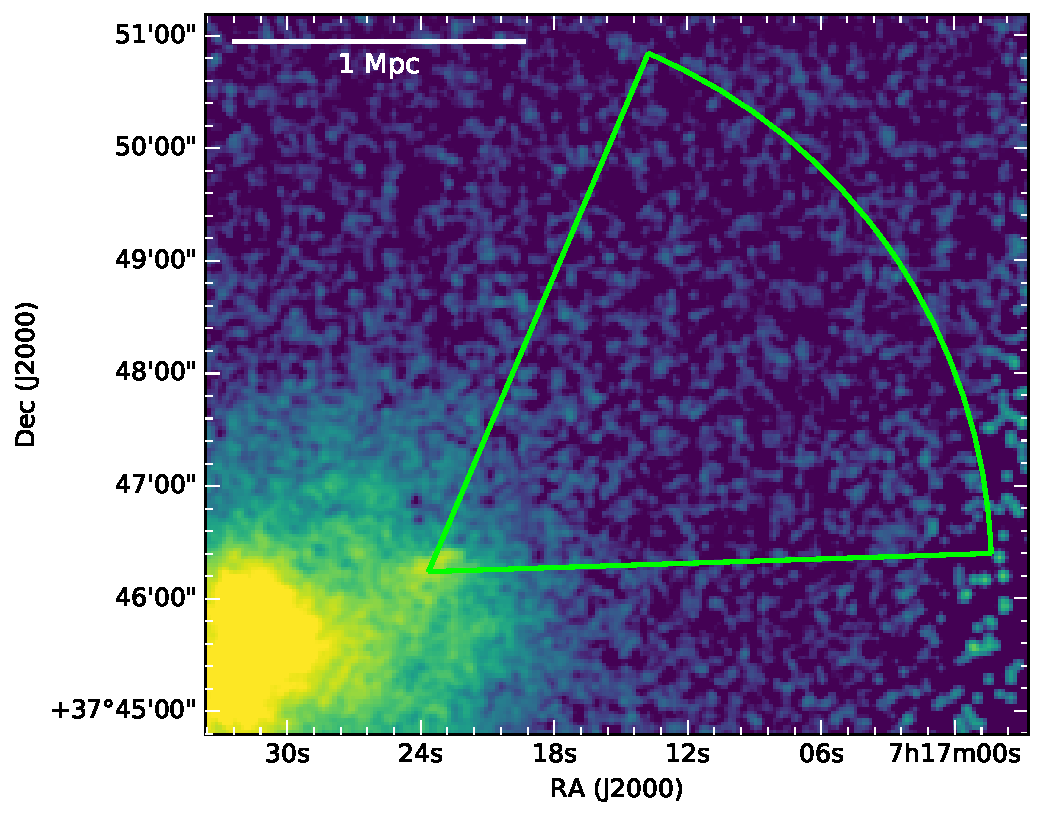
\includegraphics[width=\columnwidth]{plots/circ-panda.pdf}
    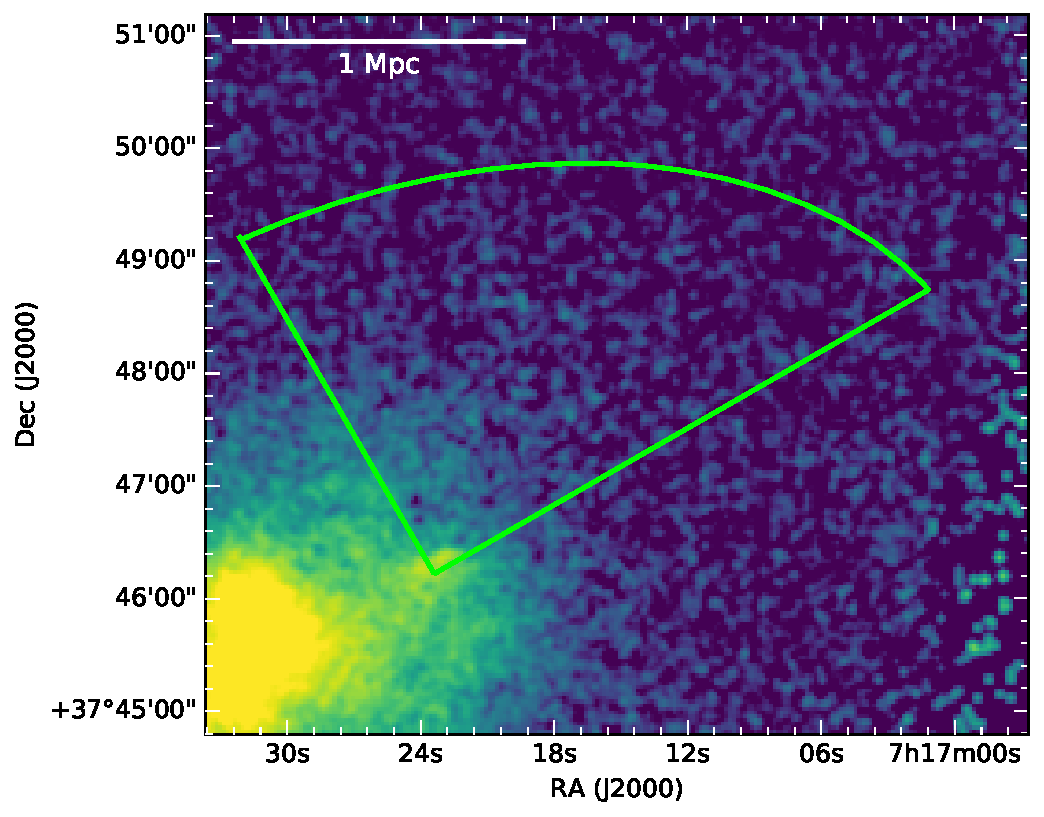
\includegraphics[width=\columnwidth]{plots/ell-panda.pdf}
    \includegraphics[width=0.33\textwidth]{plots/{macsj0717-core-circ-beta}.pdf}
    \includegraphics[width=0.33\textwidth]{plots/{macsj0717-core-ell-beta}.pdf}
    \includegraphics[width=0.33\textwidth]{plots/{macsj0717-core-ell-bknpow}.pdf}
    \caption{\emph{Left:} Chandra $0.5-4$~keV surface brightness map of MACS J0717.5+3745, showing the features discussed in this work. The image was exposure- and vignetting-corrected. Point sources were subtracted and the gaps were filled by sampling the regions surrounding the point sources.\footnote{The gaps were filled to create a more visually appealing figure. However, the imaging analysis was done on images that did not have the gaps filled. The images used in the analysis are available online as supporting material.} \emph{Right:} Regions used in the spectral analysis. The regions of main interest are drawn in solid lines, while the regions used to characterize the contaminating/surrounding emission are drawn in dashed lines. The best-fitting parameters obtained for the gas in these regions are listed in Table~\ref{tab:spectra}. \label{fig:fil}}
\end{figure*}

Approximately 670 kpc NW of the cluster center, there is a bright X-ray core with a tail extending $\sim 200$~kpc towards SE, roughly in the direction of the large-scale filament discussed in Section~\ref{sec:Filament}. This morphology suggests that this core, seen `flying' through the ICM of MACS~J0717.5+3745 and ram-pressured stripped by the cluster's dense ICM, traveled NW along the SE filament and is seen after it traversed the brightest ICM regions. In essence, the core is a later stage of the group currently seen within the filament. 

The core is still embedded (at least in projection) in the ICM of MACS~J0717.5+3745. To determine the core's physical properties, we  modeled the contamination from the ICM by extracting spectra N and S of the core. These spectra were modeled with a thermal component with a metallicity of 0.2 solar. We assumed the spectral properties were the same in the N and S regions. The spectra of the core were modeled as the sum of emission from the contaminating ICM and from the core itself. The spectra of the core and of the regions N and S of it were modeled in parallel. The best-fitting results are summarized in Table~\ref{tab:spectra}. The temperature of the core, $6.82_{-1.36}^{+1.88}$~keV, is consistent with the temperatures N and S of the core, in regions that are approximately at the same distance from the cluster center as the core. We also compared the core temperature with the temperatures ahead of (NW) and behind (SE) the core. The temperature decreases from $10.89_{-1.27}^{+2.05}$~keV behind the core, to $5.06_{-0.98}^{+1.61}$~keV ahead of the core. From these temperature measurements, we therefore find no evidence of a particularly cold core or of a temperature discontinuity (either a shock or a cold front) ahead of the core. 

A cold front and a shock front would be expected ahead of the core, similarly to the features seen in the Bullet Cluster \citep{Markevitch2002} and in front of the group NGC 4839 infalling into the Coma Cluster \citep{Neumann2001} ***other citation needed here for the cold front***. We searched for possible evidence of a cold/shock front by fitting the surface brightness profile of the group with a broken power-law density model. However, our imaging analysis did not reveal a density discontinuity significant at the $1\sigma$ confidence level. Nevertheless, we cannot exclude the existence of a density discontinuity in front of the core. The small size of the core and the additional substructure in the ICM make the modeling difficult despite \emph{Chandra}'s high spatial resolution. Furthermore, the core could be moving in a direction away from the plane of the sky, which would make the detection of a density discontinuity even more challenging; indeed, if the core originated from the large-scale filament, its movement is unlikely to be in the plane of the sky.


